\documentclass{report}
% LaTeX Template for short student reports.
% Citations should be in bibtex format and go in references.bib
\usepackage[top=3cm, bottom=3cm, left = 2cm, right = 2cm]{geometry}
\geometry{a4paper}
\usepackage[utf8]{inputenc}
\usepackage{textcomp}
\usepackage{graphicx}
\usepackage{amsmath,amssymb}
\usepackage{bm}
\usepackage[pdftex,bookmarks,colorlinks,breaklinks]{hyperref}
\hypersetup{linkcolor=black,citecolor=black,filecolor=black,urlcolor=black} % black links, for printed output
\usepackage{memhfixc}
\usepackage{pdfsync}
\usepackage{fancyhdr}
\pagestyle{fancy}
% Packages
\usepackage{titlesec}
\usepackage{lipsum}
\usepackage{verbatim}
\usepackage{subcaption}
\usepackage{float}
\def\code#1{\texttt{#1}}
%\setcounter{tocdepth}{3}
%\setcounter{secnumdepth}{3}


% Title page
\title{C1: Research Computing}
\author{Max Talberg}
\date{\today}

\begin{document}
\maketitle
\tableofcontents
\pagebreak

\section{Introduction}
This short report presents the development process of a sudoku solver python project.
The emphasis of this project is to implement good software development practices inconjunction with the development code.
As such this report will detail these processes and the challenges faced in their implementation.


- Objectives and Scope

\section{Algorithm Design and Prototyping}
-Conceptualization of the Solution

The first step before diving into the algorithm design was to conceptualise the project as a whole including the software development.
This protoyping process began on pen and paper leading to a high level workflow, the larger software development cycle (LSDC).
This cycle contains all of the steps involved in good software development practices, from the initial planning to the final deployment.
From the LSDC the prototyping logic to be was extracted and looked at in more detail to generate the protoyping logic, which is to be coded.

% protoyping images
\begin{figure}[htbp]
    \centering
    \begin{subfigure}[b]{0.14\textwidth}
        \centering
        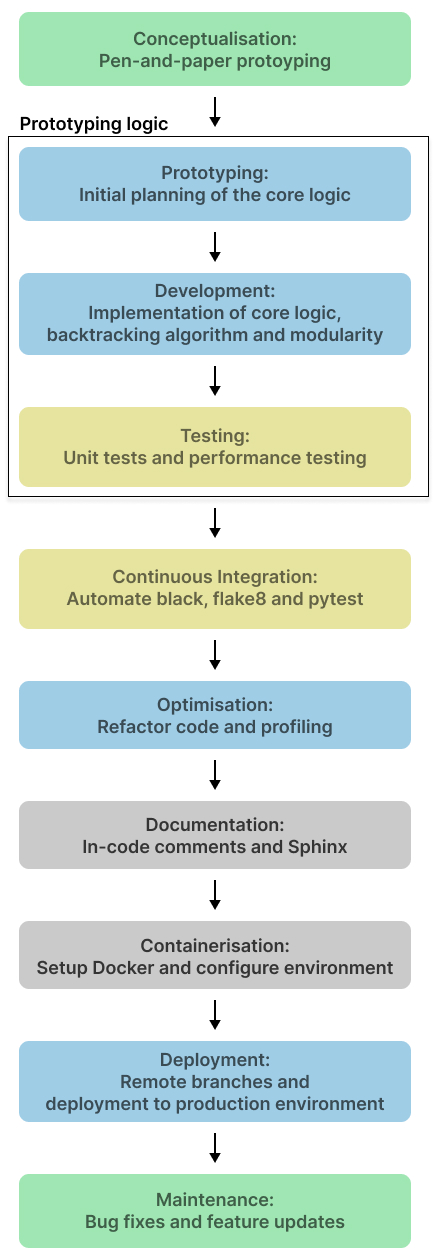
\includegraphics[width=\textwidth]{Images/SDLC.jpg}
        \caption{LSDC}
        \label{fig:figure1}
    \end{subfigure}
    \hfill
    \begin{subfigure}[b]{0.84\textwidth}
        \centering
        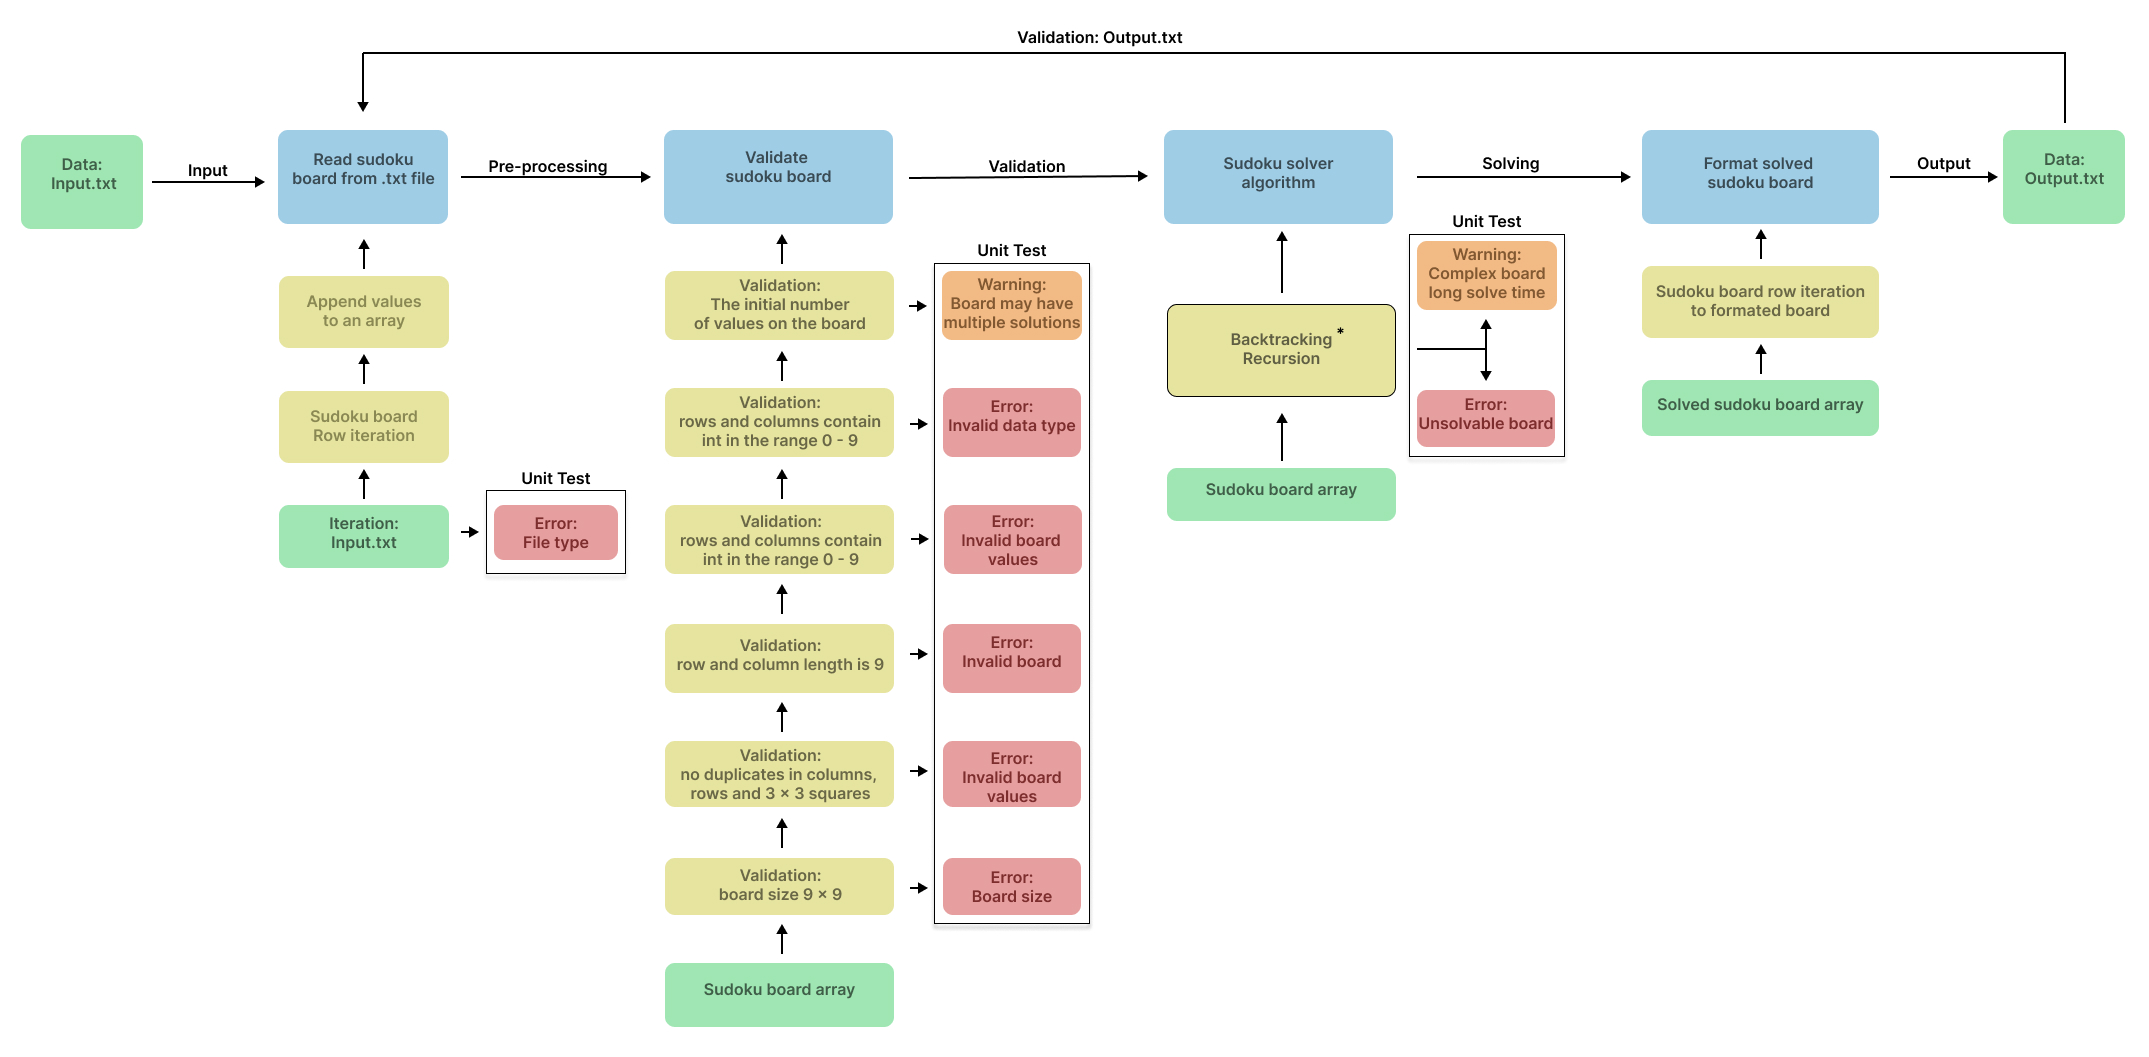
\includegraphics[width=\textwidth]{Images/prototyping.jpg}
        \caption{Prototyping logic}
        \label{fig:figure2}
    \end{subfigure}
    \caption{(a) High level prototyping of the entire project.
    Including development of the core logic and the LSDC. (b) Detailed prototyping of the core logic to be coded.}
    \label{fig:both_figures}
\end{figure}

The first step when implementing the prototyping logic is to understand the constraints and laws of sudoku.
This project is built on the following classic rules of sudoku\cite{1}:
The objective is to fill a 9 x 9 gird with digits so that each column, row and 3 x 3 subgrid contains all the digits from 1 to 9.
No digit can be repeated in any of the above mentioned areas.
A good sudoku puzzle has only one solution and the minimum number of clues is 17 \cite{2}.


The coding process began in a singluar python file, containing functions to read the text file, solve the sudoku and print the output.
These functions became more complex with the addition of error handling and classes leading to the firt release branch.
Later optimisation to improve modularity and clarity led to this one class being split up into
four seperate classes: reading the text file contating the soduko puzzle,
validating the contents of the sodoku puzzle, solving the sudoku puzzle and formatting the sudoku puzzle for the desired output.
Generating these four classes in individual files greatly improved the readbality of the project
and allowed for easier optimisation as the elements were seperated.


\subsubsection*{Read sudoku board}
This class handles the reading of a sudoku board from a text file and initialises the sudoku board as a list of lists for further processing.

\subsubsection*{Validate sudoku board}
This class handles the validation process of the sudoku board from a 2D list and converts the board to integers.
This class initially converts the 2D list of strings into integers, then iterates through the sudoku puzzle
to check the rules of sudoku are met. If these conditions are satisfied the class returns True which allows the solving process to begin.

\subsubsection*{Solve sudoku board: Backtracking}
This class handles the solving process of the sudoku board via a backtracking
algorithm. Assuming the validation was succesful this class converts a clean unsovled 2D list to a solved 2D list.
Based on the previously mentioned rules the core logic to solve a sudoku was implemented in Python following a backtarcking algorithm,
backtracking mirrors a brute force approach in that it also searches for a solution by systematically traversing the sudoku grid.
Based on the rules of sudoku, there is a limited number of possible values for each cell in the grid.
The algorithm iterates through numbers 1 to 9 and checks if the number is valid in the current cell.
If a number is valid, the algorithm moves to the next cell and repeats the process.
When a number is not valid, the algorithm backtracks to the previous cell and tries the next number.
This process repeats until the algorithm finds a solution or exhausts all possible values for the grid.
This is the simple backtracking algorithm implemented in the first release branch of this project.
This is a brute force approach to solving sudoku, which is not very efficient when dealing with harder puzzle.

??IMAGE OF BACKTRACKING LOGIC??


When beigning the programming I was aware that the simple backtracking was a simple algorithm and there are numerous more advanced algortihms and ways to optimise the backtracking. One method I looked into, altohugh did not have time to properly implement was adding a constraint propogation algorithm ontop of the backtracking.

Constraint propagation uses the rules of Sudoku to reduce the number of possible values for each cell in the grid.
This is done by using the constraints of sudoku to eliminate the invalid values for each cell, leaving a reduced number of possible values.
Paired with backtracking this algorithm can solve harder puzzles more efficiently. The constrainsts is effectivley guiding the backtracking to areas where solutions are more likely to be found. As is later evident this is useful on harder puzzles.

\subsubsection*{Format sudoku board}
This class handles the final formatting of the board, ittakes the solved 2D list
and iterativley generates the desired output to be printed onto the console.


\section{Development and Unit Testing}
This section will take a closer look at the development process and unit testing.

\subsubsection*{Read sudoku board}
During earlier development stages I had error handling in this section, since the data was read in iterativley
it seemed computationally cheaper to check for invalid characters or row length at this stage.
Although the problem with this was I could only check errors in rows as this matched the import style here,
so columns had to be done sepratly during validation. This also ncreased the number of operations
the reading fucniton is performing, I decied to keep these seprate it is a more modular approach and that the computational cost of doing these seperately is low.
In the final version this class only reads in the text file and returns a 2D list of strings. Strings becasue the processing happens in the next step.
Potential errors at this stage are the file could not exist, the file could not be a text file or the text file is empty.
These erros ar flagged as Runtime errors in the code and setup as unit tests.
Following the reorganisition of the signalur class to four classes in seperate files the unit test went through the same process.

\subsubsection*{Validate sudoku board}
As mentioned this class initially only handled erros to do with the columns, altohugh after refactiring a
modular appraoch this handles all of the validation based on the rules of sudoku. THis class cataches the most errors.
The class checks the rules of sudoku are being followed, this means the board only contains valid ingitgers in the range 1 to 9, 0 being an empty square.
That there are no duplicates in any row, column or 3 x 3 sqaure.
The class tests for aditional edge cases such as an invalid board size,
an invalid board which is a text file that doesnt contain a board and aditional checks the board converts a 2D list of strings to one of integers as expected.

After completing all of the edge cases that serve as an invalid board it became clear there are certain scenarios that the solver should be aware of and raiser a wanring but not stop the code due to error. As mentioned before a good sudoku consists of at least 17 initial values, the reason for this is that this could lead to multiple soloutions. To investage this claim I generated a time complexity plot detailing how long my solver took to solve the same sudoku puzzle while varying the number of empty squares. The general trend revealed the time taken to solve the puzzles increases with the number of empty cells. At a speficic point (around 52 empty cells) there is a susbstaintial increase in time taken for the algorithm ot solve puzzles, additionally crictical threshold at 52 serves to indicates here the puzzle soloutions stopped being unique. There is clearly less variability at this puzzle complexity forcing the backtracking algorithm to deeper levels of recursion. After 61 empty cells the time taken significacntly drops, potentially because there are so few cells that some of the many solutions are more accesible via the backtracking algorithm.

This short investiagtion was perofrmed on a singular dataset \cite{9} and in other scenarios a difficult puzzle could be set up in a way that backtracking from the top left to the bottom right works fast. Although this graph gave practical insight on the perforamnce charactierstics of sudoku at high elvels of an empty board.

\begin{figure}[H]
    \centering
    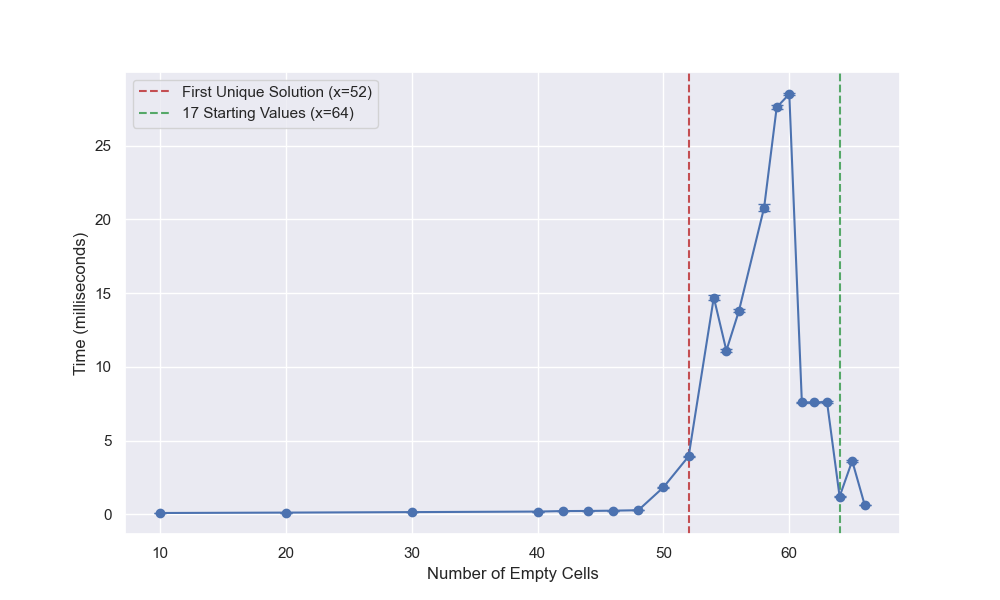
\includegraphics[width=0.8\textwidth]{Images/time_complexity.png}
    \caption{Time complexity of the backtracking algorithm}
    \label{fig:time_complexity}
\end{figure}

Based on this analysis and on good sudoku guidlines I implemented a warning under the conditions that there are less than 17 starting starting values or zero starting values (empty board).
This code still runs, it will just overide a warning that there could be multiple solutions.


\subsubsection*{Solve sudoku board: Backtracking}
The algorithmic part of the code has few error handling instances as it is assumed at this point
the 2D list of list of integers has been validated apropriatly and the baord is clean.
The unit tests for this algortihm are to confirm the backtracking algorithm is behaving as expected
in identifying possible squares. There is a further unit test checking that the solver returns the expected value for a knwon soloution.

During this development I utilised a combination of mocking and imorting sudoku boards form a data file.
Mocking was used to isolate from data and confirm i get the expected vlaues. Importing data files was used in outher instances
as this mirrors the application of this and kept the unit test files tidy.


\subsubsection*{Format sudoku board}
This class was initially a function within the validation step as this funciton was responsible for all the bnoard opetarions.
Although, to keep funcitons modular and clean i decided to follow the initial prototype process and create a seperate class.
This function iterativley geneerates the desired output from a solved 2D list of integers.
The unit test here is to determin if the format class can take a solved board and provide the expected string output for the terminal.
This test used a mocking to isolate the unit test to just the formatting class.

- Building and Refining the Core Algorithm
The algorithm was initially implemented in Python as functions, this later became a class to improve modularity and reusability.
Once the backtracking algorithm was implemented, the next step was coding a function to read the puzzle from a text file.

\subsubsection*{Continuous Integration}
The use of Continuous Integration (CI) early on in the coding process proved to be incredibly useful.
CI is a verification process that autamtically builds and tests ones code during each integration to a central repository.
In this code CI was inegrated using pre-commit hooks and I used black, flake8 and pytest.
Black is a code formatter that follows the PEP8 style, a commonly used coding style. Flake8 does a similar thing checking for styling issues.
Pytest autamtically runs the unit test, this creates continuous testing everytime one commits.
CI helps detect bugs early on in the development process, before they are impossible to find.
Integrating of CI meant wuaklity was maintained during development.
This was parotucalry useful when creating four classes from the orignal one, it helped speed up the integration process.

Setup CI meant that each commit all my unit tests woudl run and the formatting and coding style of was checked.
This ensured any bugs were caught qucikly and consistent quaiity of code was mainitend for the duartion of the project,
facilitating smooth integration when eveloping more classes.

- Implementing and Executing Unit Tests

- Continuous Integration (CI) Setup

\section{Advanced Experimentation and Refinement}

Optimisation and profiling

\subsubsection*{Exploring Edge Cases and Complex Scenarios}
When inititally desiging the unit tests the obvious things to test was if the rules are being followed. My code catches these errors and returns an error message specifiying where this happend.
Although a combination of braistorming and research \cite{3} helped determin some edge cases.
Edge cases that are related to the handling of a sudoku board included the dimensions of the board being incorrect (different to 9 x 9),
the board contaings an invalid character a number outside of 0 to 9 or a string.
As previously mentioned a good baord has at least 17 starting values, any less than this can lead to multiple soloutions.
To handle this issue i implemented a warning to be thrown under the circumstance there are less than 17 starting numbers or the board is empty.
An additional feature i could look into is giving back how many soloutions there are and what these are.
Another edge case i looked at is that of an unsolvable board, this is acheived when the algorithm has tried every square via backtracking and will return an value error saying the board is unsolvable.
Other edge cases include the input text file not being a text file or completley empty or containinng text. My code handles these and provides a specific errror message.

Fortunatly the compuatational speed fo solving a sudoku is cheap adn this is a quick process, whcih means i cna afford to unit test with each commit.
Although some more complex projects this is not possible and therefore it is harder to test logic and in such cases isolating the working parts is recommended.
I did this in a few instncces by using mocking in the unit tests as well as splitting up the code into four files each containing a different class.

\subsubsection*{Iterative Development and Branch Management}
Utlisiing git with the built in CI meant a high qualkity of code was maintianed during development.
Furhter to this untioising branches when developing features or experimenting on use cases meant there is no risk of corrupting the work acheived so far.
Utlising git and CI ensured development was smooth. When nearing completion of the project I implemnted release branches to keep track of the versions of code.
It can be seen in the first release branch that there is one file in the src folder that contained one class with all the code.
In the next version one can see this is split across four files in the src and tests folders. Utiklising version control here allows continous development whilst maintaiining rpeviusu woirk done.

\subsubsection*{Flask}
As a small extension I investigated developing a simple user interface to the sudoku solver.
This involves developing a html file detailing the layout of the interface.
I went for a simple layout with only an option to choose or drag a file, an upload button which upl,oads that text file to the screen on a sudoku board adn finally a solve button.
THis solve button solves the sudoku and shows the final answer on screen, error codes also show up if activated.
An extension if i had more time would be to integrate an animation of the backtracking process or allow more customisation and edge cases to be fucnitonal.

% app images
\begin{figure}[htbp]
    \centering
    \begin{subfigure}[b]{0.45\textwidth}
        \centering
        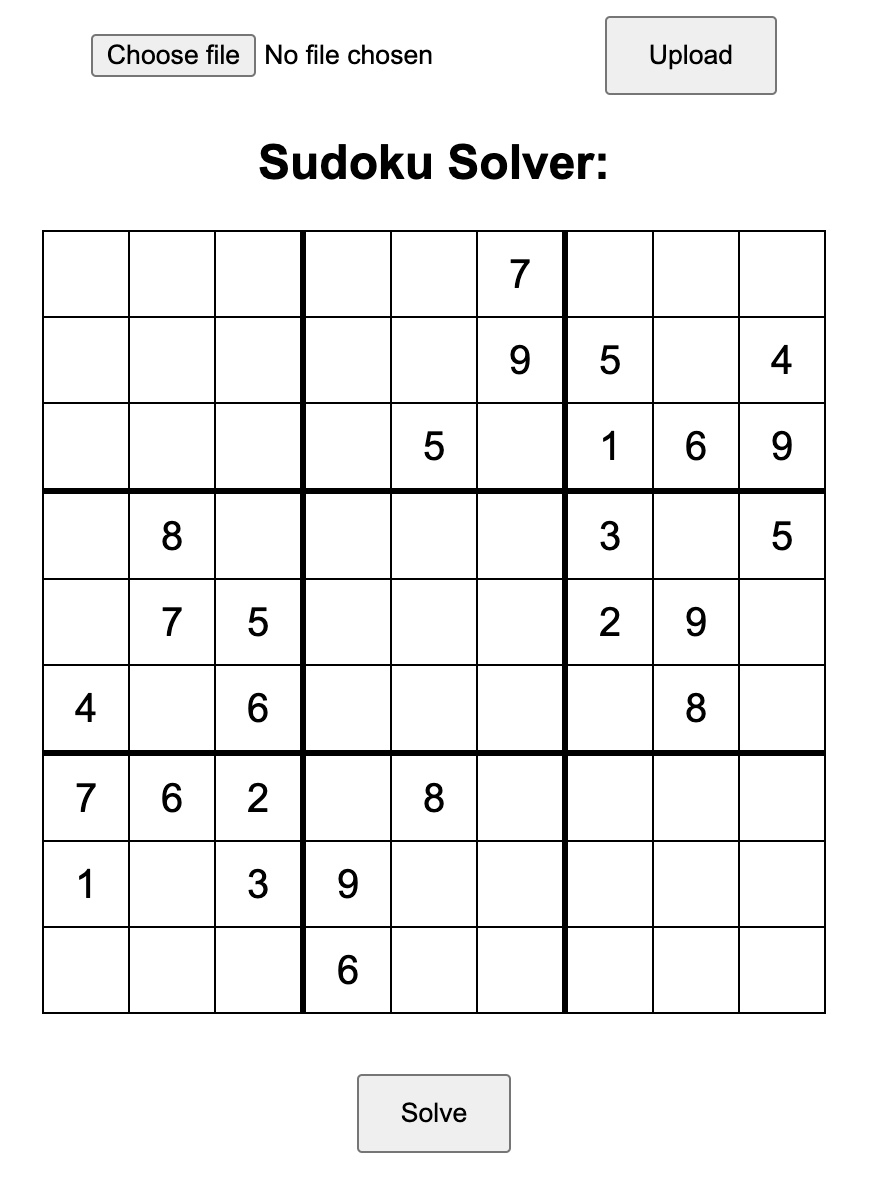
\includegraphics[width=\textwidth]{Images/app.png}
        \caption{Uploaded puzzle}
        \label{fig:figure3}
    \end{subfigure}
    \hfill
    \begin{subfigure}[b]{0.45\textwidth}
        \centering
        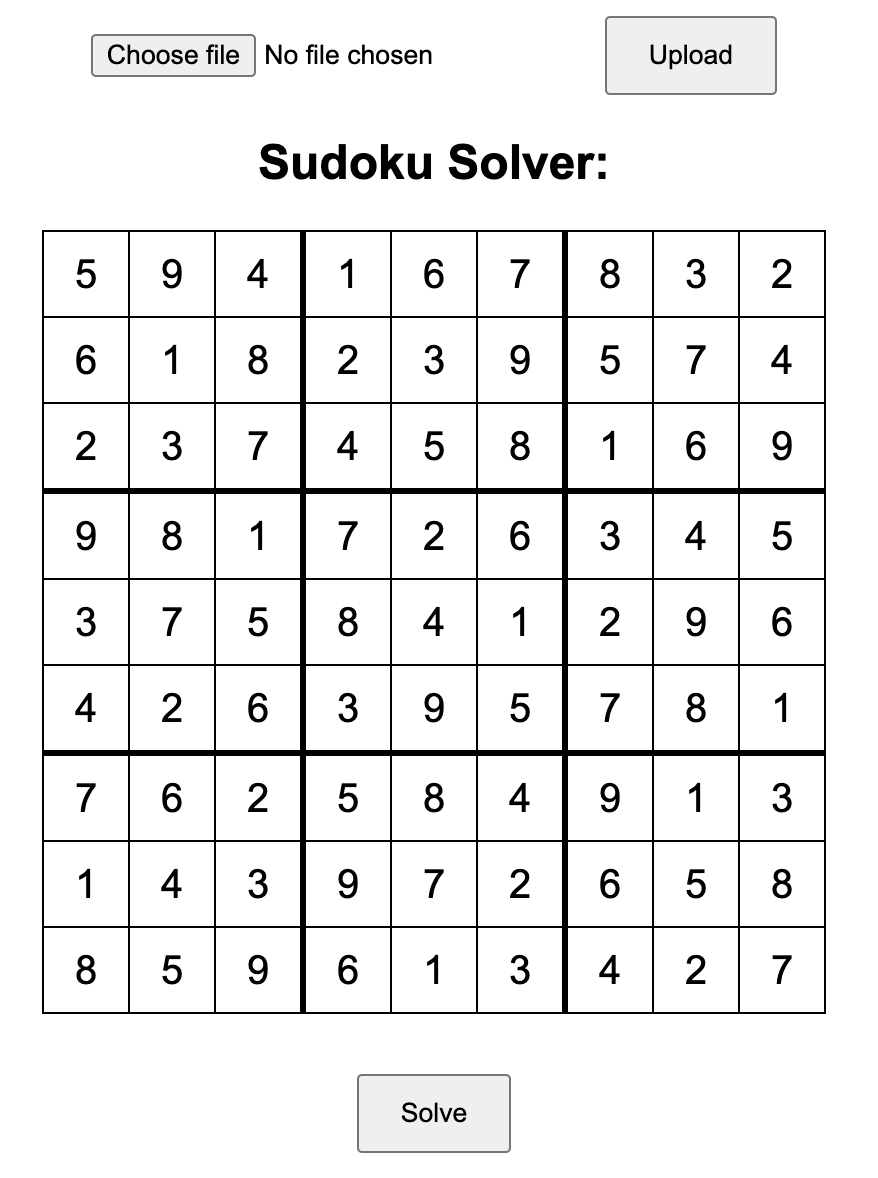
\includegraphics[width=\textwidth]{Images/appSolved.png}
        \caption{Solved puzzle}
        \label{fig:figure4}
    \end{subfigure}
    \caption{ The user interface for the sudoku solver before and after a puzzle is solved.}
    \label{fig:both_figures2}
\end{figure}

\subsubsection*{Performance Profiling and Optimisation}
Profiling and optimisation are processes used to speed up effciency in the code. The profiling and optimisation process took place adter i had released version one.
I applied a line profiler and memory profiler to investigate the time and memory complexitiies of my functions.

Developing the validation code I initially had three seperte iterations for checking if there were duplicates in the rows, columns or 3 x 3 squares.
When optimsing the code by moving all of the validation steps into the same fucntion it occured i could perform these in the same iteration.
Implemented more uses of list comprehension Clearly solving a sudoku is not a massivley expensive task, although on more comlex projects this Optimisation cnab be paramount as one scles up.

Time complexity investigation
\begin{table}[ht]
\centering
\begin{tabular}{l|r}
\hline
\textbf{puzzles\_kaggle} & \textbf{puzzles/sec} \\
\hline
rc\_mt942v3 & 362,635.9 \\
fsss \cite{4} & 1,477,910.9 \\
jczsolve \cite{5} & 597,074.2 \\
sk\_bforce2 \cite{6} & 1,234,240.0 \\
\hline
\end{tabular}
\caption{Performance comparison of different Sudoku solvers.}
\label{tab:sudoku_performance}
\end{table}


The above table is an investigation into performance on a benchmark Kaggle data set \cite{7} of 1,000,000 sudoku puzzles. This data set shows the sudoku solver performs well on a selection of easy puzzles. However, when we compare this to more difficult data, the Magic Tour Top 1465 is another common benchmark data set \cite{8} consisting of hard puzzles. The performance of our solver doesn't match up.

\begin{table}[ht]
\centering
\begin{tabular}{l|r}
\hline
\textbf{puzzles\_magic\_tourtop1465} & \textbf{puzzles/sec} \\
\hline
rc\_mt942v3 & 99999 \\
fsss2 & 69,752.5 \\
jczsolve3 & 77,888.4 \\
sk\_bforce2 & 86,535.4 \\
\hline
\end{tabular}
\caption{Performance comparison of different Sudoku solvers.}
\label{tab:sudoku_performance}
\end{table}

Investigation into why this might be happening using the inbuilt \code{\%timeit} operation. From this it became clear the bottleneck of the code as expected is the backtracking algorithm. Reading, validating and formatting all took nanoseconds, whereas the algorithm class took microseconds. This was investigated on an easy sudoku puzzle \cite{9}.  An optimisiation with more time would be to develop the backtracking algorithm by itroducing contstraints when selecting a square to backtrack on.

\section{Packaging and Usability}

At the start of the project I created a conda environment to work in to seperate the dependencies used here from the from outher projects.

- Creating a Dockerfile and Environment Setup
\subsubsection*{Dockerfile and Environment Setup}
When deploying a project using Docker is recommended as this allows users on different hardware to access your code with ease. The Docker container has a file consisting of all the environmental requirements so this project runs in that same environment everywhere.

- Writing Comprehensive Documentation
\subsubsection*{Documentation}
For this project I opted to document things in Sphinx, this is because i preferred the aesthetics compared to Doxygen. Once setup Sphinx was integrated to my code and would autmatically update when ran. A more advanced option would be to a Continuous Development (CD) pipeline which autamtically rebuilds documentation after changes (once pushed) and makes the documentaion availble of GitLab. This is only possible in a public directory.

Once integrated my Sphinx documentation worked produing an index.html file where I could locally look at the documentation. This details every comments under functions and classes. The docstrings in this project follow the NumPy style, altohugh implementing \code{sphinx.ext.napoleon} in the \code{conf.py} file ensures Sphinx correctly passes this notation, Sphinx uses reStructedText (reST) as its markup language.

- Usability and Accessibility Considerations

\section{Summary and Future Work}
- Summary of Achievements
In this project we developed a functioning sudoku solver using the backtracking algorithm compatible with the classical rules of sudoku. The project began by prototyping the LDSC and core logic, this logic was then implemented into code. This basic code was later refactored into four individual classes: reading, validating, solving and formatting. Combined these classes solved a sudoku. Next the complexity of the code developed by introducing error handling within these classes. Error handling catches any reachees of the classical rules, edge cases such as bad input text and raises warning for less than 17 starting values. These errors were later integrated to unit tests to ensure the robustness of the code. Implementing CI which contained black, flake8 and pytest ensured automatic testing with every commit aiding the development process enourmasley by ensuring early bug detection and a consistenly clean working state. Once the core logic worked well alongside unit tests, the project entered an advanced experimentaion and refinment stage where I refinded the existing code by optimising the validaiton process and investigating the perforamcne of the model ona variety of benchmark datasets and compared the performance to some fast well know sudoku solvers. At this stage I also explored a simple intutiatve user interface using flask. The next steps as part of the LSDC cosntisted of refining the projects docstrings for documentation via Sphinx and developed an Image for the project in Docker with a self contained environment for easy deployment on any device.

- Reflections on the Development Process

\subsubsection*{Potential Areas for Future Improvement}
- Potential Areas for Future Improvement
The main area for imporvment and clearly the alrgest bottleneck of the project in terms of suoku performance is the backtracking algorithm. Future work woul ocnsist of implenenting constariant propogation or perhaps a different algorithm altogether.

In regards to error handling with more time id implment a more sophisticated response to handling boards with multiple solutons. Potentailly providng all of the soloutions.

The frontend I built is very simple, future plans would ensure this is better looking, it contains interactive featurs so the user could manually cahgne the input and maybe an anitmation of the baclktraing or whatebver algortihm is being used.

In regards to packaging implementing CD with the project would automatically depoly documentation and CI with Docker for contious deployment.

\section{Appendix}

From our experiments we can conclude that \ldots

\begin{thebibliography}{9}

    \bibitem{1}
    https://en.wikipedia.org/wiki/Sudoku

    \bibitem{2}
    https://arxiv.org/abs/1201.0749

    \bibitem{3}
    http://sudopedia.enjoysudoku.com/Invalid\_Test\_Cases.html

    \bibitem{4}
    https://github.com/dobrichev/fsss2

    \bibitem{5}
    http://forum.enjoysudoku.com/3-77us-solver-2-8g-cpu-testcase-17sodoku-t30470-210.html\#p249309

    \bibitem{6}
    https://github.com/GPenet/SK\_BFORCE2

    \bibitem{7}
    https://www.kaggle.com/datasets/bryanpark/sudoku

    \bibitem{8}
    http://magictour.free.fr/sudoku.htm

    \bibitem{9}
    https://gitlab.developers.cam.ac.uk/phy/data-intensive-science-mphil/c1\_assessment/mt942/-/blob/main/Instructions.md?ref\_type=heads

\end{thebibliography}


\end{document}
